\documentclass[tikz,border=4pt]{standalone}
\usepackage{amsmath}
\usepackage{tikz}
\usepackage{pgfplots}
\pgfplotsset{compat=1.18}

\begin{document}
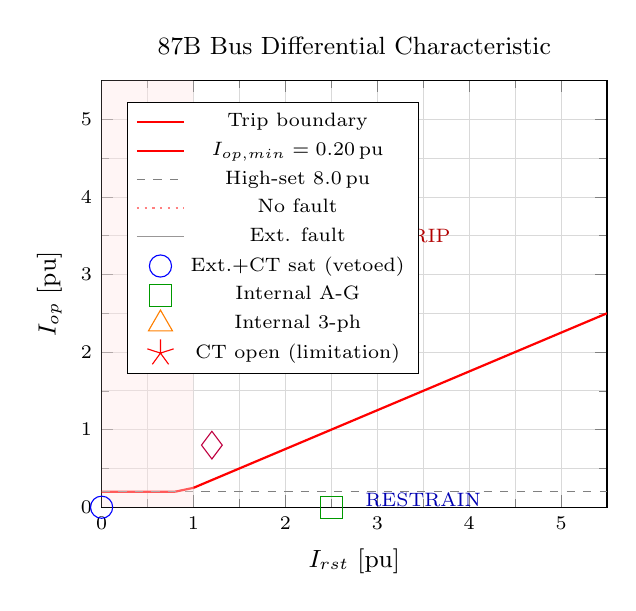
\begin{tikzpicture}
\begin{axis}[
  width=8cm, height=7cm,
  xlabel={$I_{rst}$ [pu]},
  ylabel={$I_{op}$ [pu]},
  title={87B Bus Differential Characteristic},
  xmin=0, xmax=5.5,
  ymin=0, ymax=5.5,
  grid=both,
  grid style={line width=0.3pt,gray!30},
  minor tick num=1,
  legend style={at={(0.05,0.95)},anchor=north west,font=\scriptsize},
  tick label style={font=\scriptsize},
  label style={font=\small},
  title style={font=\small},
]

%% Trip boundary: SLP1=0.25 for I_rst in [0,1], SLP2=0.50 for I_rst > 1
%% I_op_min = 0.20
\addplot[red,thick,domain=0:1,samples=50]
  {max(0.20, 0.25*x)};
\addplot[red,thick,domain=1:5.5,samples=50]
  {max(0.20, 0.25*1 + 0.50*(x-1))};
\addlegendentry{Trip boundary}

%% I_op_min dashed
\addplot[gray,dashed,domain=0:5.5] {0.20};
\addlegendentry{$I_{op,min}=0.20\,\text{pu}$}

%% High-set
\addplot[red!50,dotted,thick,domain=0:5.5] {8.0};
\addlegendentry{High-set $8.0\,\text{pu}$}

%% Shaded TRIP region (approximate, above boundary)
\addplot[fill=red!10,opacity=0.4,draw=none,domain=0:1]
  {5.5} \closedcycle;

%% Event scatter points
%% normal_load: (0,0)
\addplot[only marks,mark=o,mark size=4pt,blue] coordinates {(0.000, 0.000)};
\addlegendentry{No fault}

%% external_fault: (2.5, 0)
\addplot[only marks,mark=square,mark size=4pt,green!60!black] coordinates {(2.500, 0.000)};
\addlegendentry{Ext. fault}

%% external_fault_ct_sat: I_rst≈2.5, I_op≈4.8 (but vetoed)
\addplot[only marks,mark=triangle,mark size=5pt,orange] coordinates {(2.500, 4.776)};
\addlegendentry{Ext.+CT sat (vetoed)}

%% internal_fault_ag: I_op=6.0
\addplot[only marks,mark=star,mark size=5pt,red] coordinates {(1.500, 6.000)};
\addlegendentry{Internal A-G}

%% internal_fault_3ph: I_op=8.0
\addplot[only marks,mark=x,mark size=5pt,darkgray] coordinates {(2.000, 8.000)};
\addlegendentry{Internal 3-ph}

%% ct_open_circuit: I_op=0.8, I_rst=1.2
\addplot[only marks,mark=diamond,mark size=5pt,purple] coordinates {(1.200, 0.800)};
\addlegendentry{CT open (limitation)}

%% TRIP / RESTRAIN labels
\node[font=\scriptsize,red!70!black] at (axis cs:3.5,3.5) {TRIP};
\node[font=\scriptsize,blue!70!black] at (axis cs:3.5,0.10) {RESTRAIN};

\end{axis}
\end{tikzpicture}
\end{document}
